% Provenance (never printed): see sources/outline_sources.md (Year 1:
% astronomy of position, spherical trigonometry, time scales, insolation).
% Spherical trigonometry is absent from the mathematics series: this chapter
% owns it. Curves computed in figdata/bachelor-1/{sun_paths, day_length,
% celestial_sphere, spherical_triangle}.py (shared model _solar.py); numbers
% of the exercises and problem in the Book 3 scratch calculator ch01.py.
\chapter{Astronomi Bola}\label{ch:b1:spherical-astronomy}

Pada malam yang cerah jauh dari kota mana pun, kamera dengan pemaparan panjang yang diarahkan ke langit merekam bintang-bintang sebagai busur lingkaran, yang semuanya berpusat pada satu titik yang tidak bergerak. Bintang yang terbit di timur pukul sembilan malam ini akan terbit kira-kira pukul sembilan kurang lima besok, dan setiap malam sesudahnya sedikit lebih awal. Matahari pada tengah hari berada lebih tinggi di bulan Juni daripada di bulan Desember, dan di utara yang jauh ia tidak terbenam sama sekali pada pertengahan musim panas. Semua ini adalah rotasi Bumi dan revolusinya mengelilingi Matahari, dilihat dari permukaan tanah. Untuk menggambarkannya, ahli astronomi dan ahli geosains memerlukan koordinat pada bola, trigonometri segitiga yang digambar pada bola, serta jam yang berjalan seirama dengan bintang atau Matahari. Bab ini membangun alat-alat tersebut. Alat-alat itu kembali dalam tektonik lempeng (\cref{ch:b1:plate-kinematics}), tempat lempeng berputar pada bola, dan dalam bab-bab iklim (\cref{ch:b1:radiation-heat-transport}), tempat sinar Matahari yang diterima suatu \omterm{def:b1:spherical-astronomy:geographic}{lintang} menggerakkan angin dan arus.

\begin{recall}
Bumi berputar pada sumbunya sekali sehari dan mengelilingi Matahari sekali setahun pada orbit yang hampir berbentuk lingkaran; sumbunya miring terhadap bidang orbit, dan kemiringan inilah yang menyebabkan musim (buku-buku fisika, kelas 6 dan 12; hukum Kepler diingat kembali dari volume Sarjana Tahun ke-1 buku fisika). Sebuah titik di Bumi ditentukan oleh \omterm{def:b1:spherical-astronomy:geographic}{lintang} dan \omterm{def:b1:spherical-astronomy:geographic}{bujurnya} (Buku 1, kelas 6). Sebuah vektor berpanjang satu ditentukan oleh dua sudut, seperti pada koordinat bola; hasil kali titik dua vektor satuan adalah kosinus sudut di antara keduanya, dan hasil kali tripel $\vec u\cdot(\vec v\times\vec w)$ tidak berubah oleh permutasi siklik ketiga vektor itu.
\end{recall}

\section{Segitiga pada bola}

\begin{definition}[Lingkaran besar, segitiga bola]\label{def:b1:spherical-astronomy:spherical-triangle}
Yang disebut \emph{lingkaran besar}\index{lingkaran besar} pada bola adalah perpotongannya dengan bidang yang melalui pusat bola; setiap irisan bidang lain disebut \emph{lingkaran kecil}\index{lingkaran kecil}. Melalui dua titik yang tidak berseberangan secara diametral terdapat tepat satu lingkaran besar, dan busur yang lebih pendek dari kedua busurnya adalah lintasan terpendek di atas bola antara kedua titik itu. Yang disebut \emph{segitiga bola}\index{segitiga bola} adalah bangun yang dibentuk oleh tiga titik pada bola, titik-titik sudutnya $A$, $B$, $C$, yang dihubungkan oleh busur lingkaran besar yang kurang dari \ang{180}. Sisi-sisinya $a$, $b$, $c$ (berhadapan dengan $A$, $B$, $C$) diukur dengan sudut yang dibentuknya di pusat; sudut-sudutnya $A$, $B$, $C$ adalah sudut antara bidang-bidang sisi yang bertemu di setiap titik sudut.
\end{definition}

Pada bola berjari-jari $R$, sisi sepanjang $a$ radian memiliki panjang $Ra$. Setiap sisi dan setiap sudut terletak antara $0$ dan $\pi$.

\begin{omfigure}
\begin{tikzpicture}
\begin{axis}[x=1cm, y=1cm, hide axis, xmin=-2.7, xmax=2.7, ymin=-2.6, ymax=2.6, clip=false]
\draw[black, line width=0.6pt] (axis cs:0,0) circle (2.4cm);
\addplot[black!45, densely dashed, line width=0.4pt] coordinates {(0,0) (-0.078358,1.7847)};
\addplot[black!45, densely dashed, line width=0.4pt] coordinates {(0,0) (-1.5903,-0.2902)};
\addplot[black!45, densely dashed, line width=0.4pt] coordinates {(0,0) (1.4453,-0.16381)};
\addplot[omDef, line width=1.1pt] table {figdata/out/bachelor-1-spherical_triangle-ab.dat};
\addplot[omDef, line width=1.1pt] table {figdata/out/bachelor-1-spherical_triangle-bc.dat};
\addplot[omDef, line width=1.1pt] table {figdata/out/bachelor-1-spherical_triangle-ca.dat};
\addplot[omThm, line width=0.8pt] table {figdata/out/bachelor-1-spherical_triangle-angA.dat};
\addplot[only marks, mark=*, mark size=1.4pt] table[x=x, y=y] {figdata/out/bachelor-1-spherical_triangle-verts.dat};
\fill (axis cs:0,0) circle (1.2pt);
\begin{scope}[font=\small]
  \node[above] at (axis cs:-0.078358,1.7847) {$A$};
  \node[left] at (axis cs:-1.5903,-0.2902) {$B$};
  \node[right] at (axis cs:1.4453,-0.16381) {$C$};
  \node[above left] at (axis cs:0,0) {$O$};
  \node[omThm] at (axis cs:0.24,1.36) {$A$};
  \node[omDef] at (axis cs:0.0,-0.52) {$a$};
  \node[omDef] at (axis cs:0.95,0.95) {$b$};
  \node[omDef] at (axis cs:-1.05,0.95) {$c$};
\end{scope}
\end{axis}
\end{tikzpicture}

{\small \omterm{def:b1:spherical-astronomy:spherical-triangle}{Segitiga bola} $ABC$ pada bola dengan pusat $O$. Sisi $a$, $b$, $c$ adalah busur \omterm{def:b1:spherical-astronomy:spherical-triangle}{lingkaran besar}, yang diukur dengan sudut $BOC$, $COA$, $AOB$; sudut $A$ (merah) adalah sudut antara kedua sisi yang bertemu di $A$. Segitiga yang digambar memiliki $a = \ang{78.6}$, $b = \ang{62.6}$, $c = \ang{64.8}$ dan sudut-sudut \ang{89.9}, \ang{64.9} dan \ang{67.4}, yang jumlahnya lebih dari \ang{180}.}
\end{omfigure}

\begin{theorem}[Aturan kosinus]\label{thm:b1:spherical-astronomy:cosine-rule}
Dalam \omterm{def:b1:spherical-astronomy:spherical-triangle}{segitiga bola},
\[
  \cos a = \cos b\cos c + \sin b\sin c\cos A .
\]
\end{theorem}

\begin{proof}
Bekerjalah pada bola satuan dan pilih sumbu sehingga $A$ berada di kutub: $\vec A = (0, 0, 1)$, dan bidang $xz$ memuat $B$: $\vec B = (\sin c, 0, \cos c)$, karena $B$ berjarak sudut $c$ dari $A$. Titik $C$ berjarak sudut $b$ dari $A$, pada \omterm{def:b1:spherical-astronomy:spherical-triangle}{lingkaran besar} yang melalui $A$ dan membentuk sudut $A$ dengan bidang $xz$: $\vec C = (\sin b\cos A, \sin b\sin A, \cos b)$. Sisi $a$ adalah sudut antara $\vec B$ dan $\vec C$, sehingga
\[
  \cos a = \vec B\cdot\vec C = \sin c\sin b\cos A + \cos c\cos b. \qedhere
\]
\end{proof}

\begin{theorem}[Aturan sinus]\label{thm:b1:spherical-astronomy:sine-rule}
Dalam \omterm{def:b1:spherical-astronomy:spherical-triangle}{segitiga bola},
\[
  \frac{\sin A}{\sin a} = \frac{\sin B}{\sin b} = \frac{\sin C}{\sin c}.
\]
\end{theorem}

\begin{proof}
Dengan vektor-vektor pada bukti sebelumnya,
$\vec B \times \vec C = (-\cos c\sin b\sin A,\ \cos c\sin b\cos A - \sin c\cos b,\
\sin c\sin b\sin A)$, sehingga hasil kali tripel adalah
$\vec A\cdot(\vec B\times\vec C) = \sin b\sin c\sin A$. Hasil kali tripel tidak
berubah jika $A$, $B$, $C$ dipermutasi secara siklik; dengan menempatkan $B$, lalu $C$,
pada kutub, diperoleh dengan cara yang sama $\sin c\sin a\sin B$ dan $\sin a\sin b\sin
C$. Ketiga ungkapan itu sama; membaginya dengan $\sin a\sin b\sin c$ menghasilkan aturan tersebut.
\end{proof}

Jika sisi-sisinya kecil dibandingkan dengan jari-jari, $\cos a \approx 1 -
a^2/2$ dan $\sin a \approx a$, dan kedua aturan itu menjadi aturan kosinus dan
sinus untuk segitiga bidang: pada bagian bola yang cukup kecil, bola tampak datar.
Pada segitiga yang besar keadaannya tidak demikian: jumlah sudut suatu \omterm{def:b1:spherical-astronomy:spherical-triangle}{segitiga bola}
lebih besar dari \ang{180} (\cref{exo:b1:spherical-astronomy:12}).

\begin{method}[Jarak dan arah pada bola]\label{met:b1:spherical-astronomy:great-circle}
Untuk mencari jarak terpendek antara dua tempat dengan \omterm{def:b1:spherical-astronomy:geographic}{lintang} $\varphi_1$,
$\varphi_2$ dan \omterm{def:b1:spherical-astronomy:geographic}{bujur} $\lambda_1$, $\lambda_2$, serta arah ke mana harus berangkat:
\begin{enumerate}
  \item bentuklah segitiga dengan titik sudut kutub utara $P$ dan kedua tempat itu; sisi-sisinya dari kutub adalah kolatitud $\ang{90} -
        \varphi_1$ dan $\ang{90} - \varphi_2$, dan sudutnya di kutub adalah selisih \omterm{def:b1:spherical-astronomy:geographic}{bujur} $\Delta\lambda$;
  \item aturan kosinus memberikan jarak sudut $\Delta$:
        $\cos\Delta = \sin\varphi_1\sin\varphi_2 +
        \cos\varphi_1\cos\varphi_2\cos\Delta\lambda$; jaraknya adalah
        $R\Delta$ ($\Delta$ dalam radian);
  \item arah awal adalah sudut segitiga di tempat pertama, dari aturan kosinus yang diterapkan pada sisi di hadapannya,
        $\sin\varphi_2 = \sin\varphi_1\cos\Delta + \cos\varphi_1\sin\Delta\cos
        \mathrm{Az}$, dan diukur dari utara menuju tempat kedua.
\end{enumerate}
Arah berubah sepanjang \omterm{def:b1:spherical-astronomy:spherical-triangle}{lingkaran besar} (kecuali sepanjang meridian atau khatulistiwa): kapal atau pesawat yang mempertahankan arah kompas yang sama justru mengikuti kurva lain yang lebih panjang.
\end{method}

\section{Koordinat pada bola}

\begin{definition}[Lintang dan bujur]\label{def:b1:spherical-astronomy:geographic}
Misalkan Bumi berbentuk bola yang berputar pada sumbu kutubnya. \emph{Lintang}\index{lintang} $\varphi$ suatu titik adalah sudut antara bidang khatulistiwa dan jari-jari yang melalui titik itu, dari \ang{-90} (Kutub Selatan) sampai \ang{+90} (Kutub Utara); \emph{bujurnya}\index{bujur} $\lambda$ adalah sudut, yang diukur pada bidang khatulistiwa, antara bidang meridian titik itu dan bidang meridian acuan, yaitu meridian yang melalui Greenwich, dihitung positif ke timur, dari \ang{-180} sampai \ang{180}.
\end{definition}

Bumi sebenarnya sedikit gepeng; \omterm{def:b1:spherical-astronomy:geographic}{lintang} yang dipakai untuk peta dan untuk langit adalah sudut antara vertikal setempat dan bidang khatulistiwa, yang berbeda dari sudut geosentrik paling banyak \ang{0.2} (\cref{ch:b1:isostasy-gravity}). Garis-garis \omterm{def:b1:spherical-astronomy:geographic}{lintang} yang sama, yaitu paralel, adalah \omterm{def:b1:spherical-astronomy:spherical-triangle}{lingkaran kecil}; meridian adalah setengah \omterm{def:b1:spherical-astronomy:spherical-triangle}{lingkaran besar}.

\begin{definition}[Bola langit]\label{def:b1:spherical-astronomy:celestial-sphere}
\emph{Bola langit}\index{bola langit} adalah bola khayal yang berpusat pada pengamat, tempat setiap bintang diletakkan pada arahnya; hanya arah yang penting, bukan jaraknya. Perpanjangan sumbu Bumi bertemu dengan bola ini di \emph{kutub langit}\index{kutub langit} utara dan selatan; bidang khatulistiwa Bumi memotong bola ini sepanjang \emph{ekuator langit}\index{ekuator langit}. \emph{Zenit}\index{zenit} adalah titik tepat di atas kepala, sepanjang vertikal setempat; cakrawala adalah \omterm{def:b1:spherical-astronomy:spherical-triangle}{lingkaran besar} yang berjarak $\ang{90}$ darinya. \emph{Meridian lokal}\index{meridian lokal} adalah \omterm{def:b1:spherical-astronomy:spherical-triangle}{lingkaran besar} yang melalui zenit dan kutub langit; ia bertemu cakrawala di titik utara dan titik selatan.
\end{definition}

Ketika Bumi berputar dari barat ke timur, \omterm{def:b1:spherical-astronomy:celestial-sphere}{bola langit} tampak berputar ke arah sebaliknya, dari timur ke barat, pada sumbu \omterm{def:b1:spherical-astronomy:celestial-sphere}{kutub langit}, sekali dalam sedikit kurang dari sehari. Bintang-bintang mempertahankan posisi relatifnya: jaraknya begitu jauh sehingga perjalanan Bumi setahun mengelilingi Matahari mengubah arahnya kurang dari satu detik busur (\cref{ch:b1:observing-the-sky}).

\begin{definition}[Koordinat horizontal]\label{def:b1:spherical-astronomy:horizontal}
\emph{Tinggi}\index{tinggi (benda langit)} $h$ suatu bintang adalah sudutnya di atas cakrawala, dari \ang{-90} sampai \ang{90}; jarak \omterm{def:b1:spherical-astronomy:celestial-sphere}{zenitnya} adalah $z = \ang{90} - h$. \emph{Azimut}\index{azimut} $\mathrm{A}$-nya adalah sudut, sepanjang cakrawala, dari titik utara ke kaki vertikal bintang itu, dihitung dari \ang{0} sampai \ang{360} melalui timur.
\end{definition}

Koordinat horizontal adalah koordinat pengamat: koordinat itu berubah menurut tempat dan waktu. Koordinat langit itu sendiri dibawa oleh putaran langit.

\begin{definition}[Koordinat ekuatorial]\label{def:b1:spherical-astronomy:equatorial}
\emph{Deklinasi}\index{deklinasi (benda langit)} $\delta$ suatu bintang adalah sudutnya dari \omterm{def:b1:spherical-astronomy:celestial-sphere}{ekuator langit}, positif ke utara, dari \ang{-90} sampai \ang{90}. \omterm{def:b1:spherical-astronomy:spherical-triangle}{Lingkaran besar} yang melalui bintang dan \omterm{def:b1:spherical-astronomy:celestial-sphere}{kutub langit} disebut lingkaran jamnya. \emph{Sudut jam}\index{sudut jam} $H$ bintang adalah sudut di \omterm{def:b1:spherical-astronomy:celestial-sphere}{kutub langit} antara \omterm{def:b1:spherical-astronomy:celestial-sphere}{meridian lokal} dan lingkaran jam bintang itu, dihitung ke barat, dalam jam dengan satuan \ang{15}. \emph{Asensio rekta}\index{asensio rekta} $\alpha$ adalah sudut sepanjang \omterm{def:b1:spherical-astronomy:celestial-sphere}{ekuator langit} dari suatu titik tetap di langit, yaitu \omterm{def:b1:spherical-astronomy:ecliptic}{titik ekuinoks musim semi} (\cref{def:b1:spherical-astronomy:ecliptic}), sampai lingkaran jam bintang itu, dihitung ke timur, juga dalam jam.
\end{definition}

\omterm{def:b1:spherical-astronomy:equatorial}{Deklinasi} dan \omterm{def:b1:spherical-astronomy:equatorial}{asensio rekta} tetap di langit, seperti \omterm{def:b1:spherical-astronomy:geographic}{lintang} dan \omterm{def:b1:spherical-astronomy:geographic}{bujur} di Bumi: katalog bintang mencantumkannya. Kata deklinasi di sini hanya dipakai dalam arti astronomi ini; sudut antara utara geografis dan utara kompas selalu disebut deklinasi magnetik (\cref{ch:b1:field-lab-methods-1}).

\begin{proposition}[Dari koordinat ekuatorial ke horizontal]\label{prop:b1:spherical-astronomy:transform}
Pada \omterm{def:b1:spherical-astronomy:geographic}{lintang} $\varphi$, bintang dengan deklinasi $\delta$ dan \omterm{def:b1:spherical-astronomy:equatorial}{sudut jam} $H$ memiliki tinggi dan \omterm{def:b1:spherical-astronomy:horizontal}{azimut} yang diberikan oleh
\[
  \sin h = \sin\varphi\sin\delta + \cos\varphi\cos\delta\cos H,
  \qquad
  \cos\mathrm{A} = \frac{\sin\delta - \sin\varphi\sin h}{\cos\varphi\cos h},
\]
dengan $\mathrm{A}$ antara \ang{0} dan \ang{180} ketika bintang berada di timur meridian ($\sin H < 0$), dan $\mathrm{A} = \ang{360} - \arccos(\dots)$ ketika berada di barat. Khususnya, tinggi \omterm{def:b1:spherical-astronomy:celestial-sphere}{kutub langit} utara sama dengan \omterm{def:b1:spherical-astronomy:geographic}{lintang}.
\end{proposition}

\begin{proof}
Pertimbangkan segitiga yang dibentuk oleh \omterm{def:b1:spherical-astronomy:celestial-sphere}{kutub langit} utara $P$, \omterm{def:b1:spherical-astronomy:celestial-sphere}{zenit} $Z$ dan bintang $X$ (segitiga astronomi, atau segitiga posisi). Vertikal setempat membentuk sudut $\varphi$ dengan bidang khatulistiwa, sehingga $PZ =
\ang{90} - \varphi$; $PX = \ang{90} - \delta$; $ZX = \ang{90} - h$. Sudut di $P$ adalah \omterm{def:b1:spherical-astronomy:equatorial}{sudut jam} $H$; sudut di $Z$ adalah \omterm{def:b1:spherical-astronomy:horizontal}{azimut} bintang yang diukur dari utara (ke timur atau ke barat meridian). Aturan kosinus untuk sisi $ZX$, yang berhadapan dengan $P$, memberikan
$\cos(\ang{90} - h) = \cos(\ang{90} - \varphi)\cos(\ang{90} - \delta) +
\sin(\ang{90} - \varphi)\sin(\ang{90} - \delta)\cos H$, yaitu rumus pertama. Aturan kosinus untuk sisi $PX$, yang berhadapan dengan $Z$, memberikan
$\sin\delta = \sin\varphi\sin h + \cos\varphi\cos h\cos\mathrm{A}$, yaitu rumus kedua. Untuk kutub, $\delta = \ang{90}$ dan rumus pertama menjadi
$\sin h = \sin\varphi$.
\end{proof}

\begin{omfigure}
\begin{tikzpicture}
\pic (cs) at (0,0) {celestialsphere=45};
\begin{axis}[x=1cm, y=1cm, hide axis, anchor=origin, at={(0,0)}, xmin=-2.6, xmax=2.6, ymin=-2.4, ymax=2.5, clip=false]
\addplot[omField, line width=1.1pt] table[x=x, y=y] {figdata/out/bachelor-1-celestial_sphere-vertical.dat};
\addplot[black!80, line width=0.9pt, densely dash dot] table[x=x, y=y] {figdata/out/bachelor-1-celestial_sphere-hourcircle.dat};
\addplot[only marks, mark=star, mark size=3pt, mark options={line width=0.8pt}] table[x=x, y=y] {figdata/out/bachelor-1-celestial_sphere-star.dat};
\end{axis}
\begin{scope}[font=\footnotesize]
  \node[above] at (cs-Z) {$Z$};
  \node[above left] at (cs-NCP) {$P$};
  \node[left] at (cs-N) {U};
  \node[right] at (cs-S) {S};
  \node[below] at (cs-W) {B};
  \node[below, fill=white, fill opacity=0.8, text opacity=1, inner sep=1pt] at (cs-E) {T};
  \node[above right] at (0.2262,0.94) {$X$};
  \node[omField] at (0.55,0.2) {$h$};
  \node[omDef, right] at (2.0,-1.25) {khatulistiwa};
  \node[left] at (-2.0,-0.3) {cakrawala};
  \node at (-1.35,0.62) {$\varphi$};
\end{scope}
\draw[black!60, line width=0.4pt] (-1.05,0) arc[start angle=180, end angle=137, radius=1.05cm];
\end{tikzpicture}

{\small Langit pada \omterm{def:b1:spherical-astronomy:geographic}{lintang} \ang{45} LU, dilihat dari barat, dengan utara di sebelah kiri. \omterm{def:b1:spherical-astronomy:celestial-sphere}{Kutub langit} utara $P$ berada pada tinggi di atas titik utara yang sama dengan \omterm{def:b1:spherical-astronomy:geographic}{lintang} (merah: sumbu \omterm{def:b1:spherical-astronomy:celestial-sphere}{kutub langit}); \omterm{def:b1:spherical-astronomy:celestial-sphere}{ekuator langit} (biru) memotong cakrawala di titik timur dan barat. Sebuah bintang $X$ dengan deklinasi \ang{25}, tiga jam dua puluh menit setelah melintasi meridian (\omterm{def:b1:spherical-astronomy:equatorial}{sudut jam} \ang{50}), berada pada tinggi $h = \ang{45.3}$ (hijau: lingkaran vertikalnya, dari \omterm{def:b1:spherical-astronomy:celestial-sphere}{zenit} $Z$ ke cakrawala) dan \omterm{def:b1:spherical-astronomy:horizontal}{azimut} \ang{261}; lingkaran jamnya (strip titik-titik) membentang dari kutub, melalui bintang, sampai ekuator. Dihitung dengan \cref{prop:b1:spherical-astronomy:transform}.}
\end{omfigure}

\begin{proposition}[Kulminasi dan bintang sirkumpolar]\label{prop:b1:spherical-astronomy:culmination}
Pada \omterm{def:b1:spherical-astronomy:geographic}{lintang} $\varphi$, sebuah bintang dengan deklinasi $\delta$ melintasi meridian ($H = 0$) pada tinggi $\ang{90} - |\varphi - \delta|$, di selatan \omterm{def:b1:spherical-astronomy:celestial-sphere}{zenit} jika $\delta < \varphi$, dan di utara \omterm{def:b1:spherical-astronomy:celestial-sphere}{zenit} jika $\delta > \varphi$. Di belahan utara ($\varphi > 0$) bintang itu tidak pernah terbenam jika $\delta > \ang{90} - \varphi$, dan tidak pernah terbit jika $\delta < -(\ang{90} - \varphi)$.
\end{proposition}

\begin{proof}
Untuk $H = 0$, $\sin h = \sin\varphi\sin\delta + \cos\varphi\cos\delta =
\cos(\varphi - \delta)$, sehingga $h = \ang{90} - |\varphi - \delta|$. \omterm{def:b1:spherical-astronomy:horizontal}{Tinggi terendah}, pada $H = \ang{180}$, memenuhi $\sin h = -\cos(\varphi + \delta)$; nilainya positif jika $\varphi + \delta > \ang{90}$. Bintang tetap berada di bawah cakrawala jika bahkan tinggi tertingginya pun negatif,
$|\varphi - \delta| > \ang{90}$.
\end{proof}

\begin{definition}[Bintang sirkumpolar]\label{def:b1:spherical-astronomy:circumpolar}
Yang disebut \emph{bintang sirkumpolar}\index{bintang sirkumpolar} adalah bintang yang tidak pernah terbenam pada \omterm{def:b1:spherical-astronomy:geographic}{lintang} pengamat: ia berputar mengelilingi \omterm{def:b1:spherical-astronomy:celestial-sphere}{kutub langit}, melintasi meridian di atas kutub dan, dua belas jam sideris kemudian, di bawahnya.
\end{definition}

\begin{omfigure}
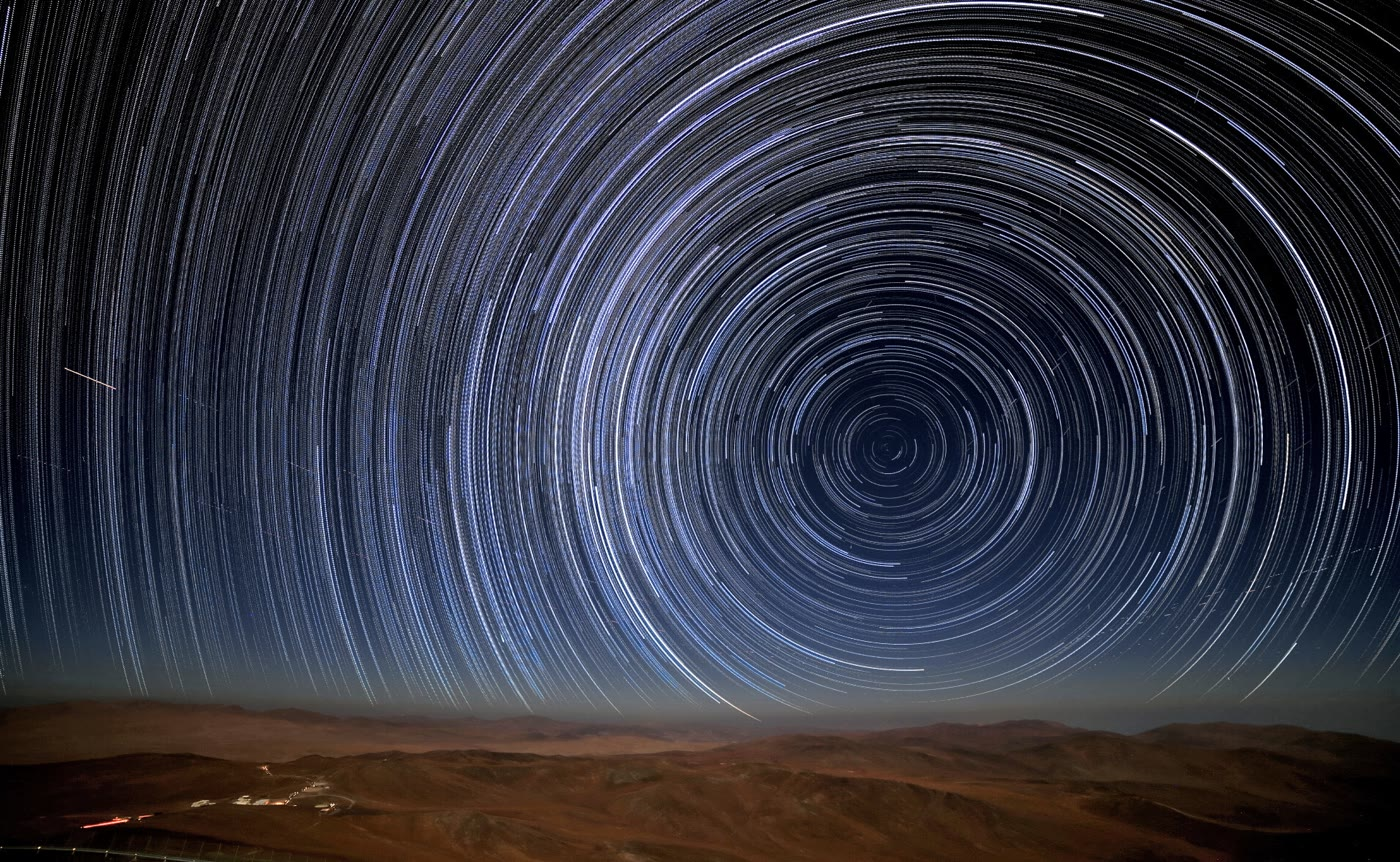
\includegraphics[width=0.8\linewidth]{images/book3/b1-star-trails-paranal.jpg}
% ledger: commons:eso-paranal-star-trails, mpc:paranal

{\small Jejak bintang di atas Observatorium Paranal, di gurun Atacama, pada \omterm{def:b1:spherical-astronomy:geographic}{lintang} \ang{24.6} LS: pemaparan panjang merekam busur setiap bintang di sekeliling \omterm{def:b1:spherical-astronomy:celestial-sphere}{kutub langit} selatan, yang berada \ang{24.6} di atas cakrawala selatan. Foto R.~Wesson/ESO, CC BY 4.0.}
\end{omfigure}

\section{Waktu sideris dan waktu matahari}

\begin{definition}[Ekliptika]\label{def:b1:spherical-astronomy:ecliptic}
Yang disebut \emph{ekliptika}\index{ekliptika} adalah \omterm{def:b1:spherical-astronomy:spherical-triangle}{lingkaran besar} pada \omterm{def:b1:spherical-astronomy:celestial-sphere}{bola langit} sepanjang mana Matahari tampak bergerak dalam satu tahun, yaitu jejak bidang orbit Bumi. Ekliptika miring terhadap \omterm{def:b1:spherical-astronomy:celestial-sphere}{ekuator langit} sebesar \emph{kemiringan ekliptika}\index{kemiringan ekliptika} $\varepsilon$, yaitu kemiringan sumbu Bumi terhadap orbitnya. Ekliptika memotong ekuator di dua titik; \emph{titik ekuinoks musim semi}\index{titik ekuinoks musim semi} $\gamma$ adalah titik tempat Matahari melintasi ekuator ke utara, pada bulan Maret. \omterm{def:b1:spherical-astronomy:geographic}{Bujur} ekliptika Matahari $\lambda_\odot$ adalah sudutnya sepanjang ekliptika dari $\gamma$, dihitung ke timur.
\end{definition}

% ledger: earth:obliquity (23.44)
Kemiringan itu kini $\varepsilon = \ang{23.44}$.

\begin{definition}[Waktu sideris]\label{def:b1:spherical-astronomy:sidereal-time}
\emph{Waktu sideris}\index{waktu sideris} setempat adalah \omterm{def:b1:spherical-astronomy:equatorial}{sudut jam} \omterm{def:b1:spherical-astronomy:ecliptic}{titik ekuinoks musim semi} $\gamma$. Hari sideris adalah selang antara dua lintasan $\gamma$ melalui meridian.
\end{definition}

Karena \omterm{def:b1:spherical-astronomy:equatorial}{asensio rekta} dihitung ke timur dari $\gamma$ dan \omterm{def:b1:spherical-astronomy:equatorial}{sudut jam} ke barat dari meridian, untuk setiap bintang
\[
  H = \mathrm{LST} - \alpha ,
\]
dengan LST adalah \omterm{def:b1:spherical-astronomy:sidereal-time}{waktu sideris} setempat: sebuah bintang melintasi meridian ketika \omterm{def:b1:spherical-astronomy:sidereal-time}{waktu sideris} sama dengan \omterm{def:b1:spherical-astronomy:equatorial}{asensio rektanya}. Jam observatorium yang menunjukkan \omterm{def:b1:spherical-astronomy:sidereal-time}{waktu sideris} memberi tahu sekilas bagian langit mana yang berada di atas kepala.

\begin{proposition}[Hari sideris dan hari matahari]\label{prop:b1:spherical-astronomy:sidereal-day}
Dalam satu \omterm{def:b1:spherical-astronomy:tropical-year}{tahun tropis} yang berisi $N$ hari matahari rata-rata, Bumi berputar $N + 1$ kali terhadap bintang-bintang. Maka hari sideris berlangsung
\[
  \frac{N}{N + 1}\times\qty{24}{h},
\]
dan dengan $N = 365.2422$ ini sama dengan \qty{23}{h}~\qty{56}{min}~\qty{4.09}{s}: sebuah bintang melintasi meridian \qty{3}{min}~\qty{56}{s} \omterm{def:b1:spherical-astronomy:solar-time}{waktu matahari rata-rata} lebih awal setiap hari.
\end{proposition}

\begin{proof}
% ledger: usno:tropical-year, earth:Trot (23.9345 h)
Hitung putaran relatif terhadap Matahari dan relatif terhadap bintang selama satu tahun. Matahari bergerak sekali mengelilingi \omterm{def:b1:spherical-astronomy:ecliptic}{ekliptika} ke timur dalam setahun, searah dengan rotasi Bumi. Relatif terhadap Matahari, Bumi karena itu membuat satu putaran lebih sedikit daripada relatif terhadap bintang-bintang: $N$ hari matahari dan $N + 1$ hari sideris mengisi tahun yang sama. Hari sideris adalah $N/(N+1)$ hari matahari, yaitu $\qty{86400}{s}\times 365.2422/366.2422 = \qty{86164.09}{s}$; selisihnya adalah $\qty{235.9}{s}$. Hasil ini sesuai dengan periode rotasi Bumi yang diukur terhadap bintang-bintang, \qty{23.9345}{h}.
\end{proof}

\begin{definition}[Waktu matahari]\label{def:b1:spherical-astronomy:solar-time}
\emph{Waktu matahari semu}\index{waktu matahari semu} adalah \omterm{def:b1:spherical-astronomy:equatorial}{sudut jam} Matahari ditambah 12 jam: jam matahari menunjukkannya, dan saat tengah hari adalah ketika Matahari melintasi meridian. \emph{Waktu matahari rata-rata}\index{waktu matahari rata-rata} adalah \omterm{def:b1:spherical-astronomy:equatorial}{sudut jam}, ditambah 12 jam, dari Matahari rata-rata fiktif yang bergerak sepanjang \omterm{def:b1:spherical-astronomy:celestial-sphere}{ekuator langit} dengan laju seragam, menyelesaikan satu putaran dalam satu \omterm{def:b1:spherical-astronomy:tropical-year}{tahun tropis}. Selisihnya, semu dikurangi rata-rata, adalah \emph{perata waktu}\index{perata waktu}.
\end{definition}

Matahari sejati mendahului dan tertinggal dari Matahari rata-rata karena dua alasan. Bumi bergerak lebih cepat dekat perihelion, pada awal Januari, daripada dekat aphelion, sehingga kemajuan Matahari sepanjang \omterm{def:b1:spherical-astronomy:ecliptic}{ekliptika} tidak merata (hukum kedua Kepler); dan Matahari bergerak sepanjang \omterm{def:b1:spherical-astronomy:ecliptic}{ekliptika}, yang miring terhadap ekuator, sehingga gerak seragam sepanjang \omterm{def:b1:spherical-astronomy:ecliptic}{ekliptika} pun terproyeksi ke ekuator, yang diukur oleh \omterm{def:b1:spherical-astronomy:equatorial}{sudut jam}, secara tidak merata, lebih cepat dekat titik balik matahari daripada dekat ekuinoks. Jam sipil menunjukkan \omterm{def:b1:spherical-astronomy:solar-time}{waktu matahari rata-rata} pada meridian acuan zona waktunya; \omterm{def:b1:spherical-astronomy:solar-time}{waktu matahari rata-rata} setempat pada \omterm{def:b1:spherical-astronomy:geographic}{bujur} $\lambda$ mendahului waktu di Greenwich sebesar $\lambda/\ang{15}$ jam.

\begin{omfigure}
\begin{tikzpicture}
\begin{axis}[omrecord, width=0.9\linewidth, height=5.2cm, xmin=0, xmax=365,
  xtick={0,31,59,90,120,151,181,212,243,273,304,334,365},
  xticklabels={J,F,M,A,M,J,J,A,S,O,N,D,},
  ylabel={perata waktu (menit)}, ymin=-20, ymax=21,
  tick label style={font=\scriptsize}, label style={font=\small}]
\addplot[black!50, line width=0.4pt] coordinates {(0,0) (365,0)};
\addplot[omDef, line width=1.1pt] table[x=day, y=eot_min] {figdata/out/bachelor-1-day_length-eot.dat};
\node[font=\scriptsize, above, fill=white, inner sep=1pt] at (axis cs:306,16.6) {$+16.4$};
\node[font=\scriptsize, below, fill=white, inner sep=1pt] at (axis cs:41,-14.4) {$-14.2$};
\end{axis}
\end{tikzpicture}

{\small \omterm{def:b1:spherical-astronomy:solar-time}{Perata waktu} sepanjang tahun (\omterm{def:b1:spherical-astronomy:solar-time}{waktu matahari semu} dikurangi \omterm{def:b1:spherical-astronomy:solar-time}{waktu matahari rata-rata}): jam matahari dapat lebih cepat hingga \qty{16.4}{min} pada awal November dan lebih lambat \qty{14.2}{min} pada pertengahan Februari. Dihitung dari orbit Kepler dengan eksentrisitas 0,0167, kemiringan \ang{23.44}, \omterm{def:b1:spherical-astronomy:geographic}{bujur} perihelion, dan tanggal ekuinoks Maret 2026.}
% ledger: earth:ecc, earth:obliquity, nasa:earth-perihelion-longitude, usno:seasons-2026
\end{omfigure}

\section{Terbit, terbenam, dan Matahari}

\begin{proposition}[Terbit dan terbenam]\label{prop:b1:spherical-astronomy:rising}
Pada \omterm{def:b1:spherical-astronomy:geographic}{lintang} $\varphi$, sebuah bintang dengan deklinasi $\delta$ yang terbit dan terbenam melintasi cakrawala pada \omterm{def:b1:spherical-astronomy:equatorial}{sudut jam} $\pm H_0$ dengan
\[
  \cos H_0 = -\tan\varphi\tan\delta ,
\]
pada \omterm{def:b1:spherical-astronomy:horizontal}{azimut} $\mathrm{A}_0$ dengan $\cos\mathrm{A}_0 = \sin\delta/\cos\varphi$ (saat terbit; ia terbenam pada $\ang{360} - \mathrm{A}_0$). Ia tetap di atas cakrawala selama $2H_0$, yang diubah ke jam dengan laju \ang{15} per jam.
\end{proposition}

\begin{proof}
Pada horizon $h = 0$, dan \cref{prop:b1:spherical-astronomy:transform} memberikan $0 = \sin\varphi\sin\delta + \cos\varphi\cos\delta\cos H_0$, dan $\cos\mathrm{A}_0 = \sin\delta/\cos\varphi$. \omterm{def:b1:spherical-astronomy:equatorial}{Sudut jam} bertambah secara seragam, sebesar \ang{15} per jam, dari $-H_0$ saat terbit sampai $+H_0$ saat terbenam.
\end{proof}

Untuk Matahari, ini memberi panjang hari, jika Matahari dianggap sebagai titik dan pembiasan cahaya oleh udara diabaikan (keduanya menambah beberapa menit pada lamanya siang). Pada ekuinoks $\delta = 0$, $H_0 = \ang{90}$: siang dan malam berlangsung dua belas jam di mana-mana, dan Matahari terbit tepat di timur.

\begin{omfigure}
\begin{tikzpicture}
\begin{axis}[omrecord, width=0.85\linewidth, height=5.6cm, xmin=40, xmax=320, ymin=0, ymax=75,
  xtick={45,90,135,180,225,270,315}, xticklabels={TL,T,TG,S,BD,B,BL}, ytick={0,15,30,45,60,75},
  xlabel={azimut}, ylabel={tinggi Matahari ($^\circ$)},
  tick label style={font=\scriptsize}, label style={font=\small}]
\addplot[omThm, line width=1pt] table[x=az_deg, y=alt_deg] {figdata/out/bachelor-1-sun_paths-june.dat};
\addplot[black, line width=1pt] table[x=az_deg, y=alt_deg] {figdata/out/bachelor-1-sun_paths-equinox.dat};
\addplot[omDef, line width=1pt] table[x=az_deg, y=alt_deg] {figdata/out/bachelor-1-sun_paths-december.dat};
\begin{scope}[font=\scriptsize, fill=white, fill opacity=0.8, text opacity=1, inner sep=1pt]
  \node[omThm, above, fill=white] at (axis cs:180,68.4) {solstis Juni, $\ang{68.4}$};
  \node[above, fill=white] at (axis cs:180,45) {ekuinoks, $\ang{45}$};
  \node[omDef, above, fill=white] at (axis cs:180,21.6) {solstis Desember, $\ang{21.6}$};
\end{scope}
\end{axis}
\end{tikzpicture}

{\small Lintasan Matahari di langit pada \omterm{def:b1:spherical-astronomy:geographic}{lintang} \ang{45} LU pada solstis Juni (merah), pada ekuinoks (hitam) dan pada solstis Desember (biru), dengan \omterm{def:b1:spherical-astronomy:horizontal}{tinggi tengah hari} $\ang{90} - \varphi + \delta_\odot$. Pada ekuinoks Matahari terbit tepat di timur dan terbenam tepat di barat; pada bulan Juni ia terbit di timur laut.}
\end{omfigure}

\begin{proposition}[Deklinasi Matahari]\label{prop:b1:spherical-astronomy:sun-declination}
Ketika Matahari berada pada \omterm{def:b1:spherical-astronomy:geographic}{bujur} \omterm{def:b1:spherical-astronomy:ecliptic}{ekliptika} $\lambda_\odot$, deklinasi dan \omterm{def:b1:spherical-astronomy:equatorial}{asensio rektanya} memenuhi
\[
  \sin\delta_\odot = \sin\varepsilon\sin\lambda_\odot, \qquad
  \tan\alpha_\odot = \cos\varepsilon\tan\lambda_\odot .
\]
\end{proposition}

\begin{proof}
Ambil sumbu dengan $x$ menuju $\gamma$ dan $z$ menuju \omterm{def:b1:spherical-astronomy:celestial-sphere}{kutub langit} utara.
Pada sumbu $x$, $y'$, $z'$ yang melekat pada \omterm{def:b1:spherical-astronomy:ecliptic}{ekliptika}, dengan $z'$ menuju kutubnya, arah Matahari adalah $(\cos\lambda_\odot, \sin\lambda_\odot, 0)$. Sumbu \omterm{def:b1:spherical-astronomy:ecliptic}{ekliptika} diperoleh dari sumbu ekuator yang diputar sebesar sudut $\varepsilon$ terhadap $x$, sehingga pada sumbu ekuator arah Matahari adalah
$(\cos\lambda_\odot,\ \sin\lambda_\odot\cos\varepsilon,\
\sin\lambda_\odot\sin\varepsilon)$. Komponen $z$-nya adalah $\sin\delta_\odot$; perbandingan komponen $y$ dan $x$-nya adalah $\tan\alpha_\odot$.
\end{proof}

\begin{omfigure}
\begin{tikzpicture}
\begin{axis}[omrecord, width=0.9\linewidth, height=6cm, xmin=0, xmax=365, ymin=0, ymax=24,
  xtick={0,31,59,90,120,151,181,212,243,273,304,334,365},
  xticklabels={J,F,M,A,M,J,J,A,S,O,N,D,}, ytick={0,6,12,18,24},
  ylabel={panjang hari (h)}, tick label style={font=\scriptsize}, label style={font=\small},
  legend style={font=\scriptsize, at={(0.5,1.02)}, anchor=south, draw=none}, legend columns=5,
  legend cell align=left]
\addplot[black, line width=0.9pt] table[x=day, y=lat0] {figdata/out/bachelor-1-day_length-lengths.dat};
\addplot[omDef, line width=0.9pt] table[x=day, y=lat30] {figdata/out/bachelor-1-day_length-lengths.dat};
\addplot[omThm, line width=0.9pt] table[x=day, y=lat45] {figdata/out/bachelor-1-day_length-lengths.dat};
\addplot[omField, line width=0.9pt] table[x=day, y=lat60] {figdata/out/bachelor-1-day_length-lengths.dat};
\addplot[black, line width=0.9pt, densely dashed] table[x=day, y=lat70] {figdata/out/bachelor-1-day_length-lengths.dat};
\legend{\ang{0}, \ang{30} LU, \ang{45} LU, \ang{60} LU, \ang{70} LU}
\end{axis}
\end{tikzpicture}

{\small Panjang hari (pusat Matahari di atas horizon geometris) sepanjang tahun pada lima \omterm{def:b1:spherical-astronomy:geographic}{lintang} utara, dari
\cref{prop:b1:spherical-astronomy:rising,prop:b1:spherical-astronomy:sun-declination}.
Pada \ang{70} LU Matahari tetap di atas cakrawala selama berminggu-minggu di sekitar solstis Juni dan tetap di bawahnya di sekitar solstis Desember. Di belahan selatan kurvanya bergeser setengah tahun.}
\end{omfigure}

\begin{definition}[Insolasi]\label{def:b1:spherical-astronomy:insolation}
Yang disebut \emph{insolasi}\index{insolasi} di suatu tempat dan pada suatu saat adalah daya sinar Matahari yang diterima per satuan luas permukaan horizontal di puncak atmosfer. Dengan $S_0$ iradiansi Matahari pada jarak rata-rata $a$ Matahari, $r$ jarak sebenarnya, dan $\theta_z$ jarak \omterm{def:b1:spherical-astronomy:celestial-sphere}{zenit} Matahari,
\[
  I = S_0\left(\frac{a}{r}\right)^{2}\cos\theta_z = S_0\left(\frac{a}{r}\right)^{2}\sin h_\odot
  \quad (h_\odot > 0), \qquad I = 0 \text{ pada malam hari}.
\]
\end{definition}

% ledger: earth:TSI (1361 W/m2), earth:peri, earth:aph, earth:a
Faktor $(a/r)^2$ adalah hukum kuadrat terbalik untuk cahaya (buku-buku fisika); faktor $\cos\theta_z$ muncul karena seberkas sinar berpenampang satu meter persegi tersebar di atas $1/\cos\theta_z$ meter persegi tanah datar. Dengan $S_0 = \qty{1361}{W.m^{-2}}$ dan jarak Matahari--Bumi sebesar \qty{147.1e6}{km} pada perihelion dan \qty{152.1e6}{km} pada aphelion, faktor $(a/r)^2$ berubah sebesar $\pm\qty{3.4}{\percent}$ sepanjang tahun. Kemiringan sumbu jauh lebih menentukan: ia mengubah \omterm{def:b1:spherical-astronomy:horizontal}{tinggi tengah hari} maupun lamanya siang, dan keduanya bersama-sama menghasilkan musim. Jumlah harian dan tahunan \omterm{def:b1:spherical-astronomy:insolation}{insolasi}, yang menggerakkan iklim, dihitung dalam \cref{ch:b1:radiation-heat-transport}.


\section{Kalender}

\begin{definition}[Tahun tropis]\label{def:b1:spherical-astronomy:tropical-year}
Yang disebut \emph{tahun tropis}\index{tahun tropis} adalah selang rata-rata antara dua lintasan Matahari melalui \omterm{def:b1:spherical-astronomy:ecliptic}{titik ekuinoks musim semi}. Tahun inilah yang menentukan musim; lamanya 365.2422 hari matahari rata-rata.
\end{definition}

% ledger: usno:tropical-year, earth:Psid (365.256 d)
\omterm{def:b1:spherical-astronomy:tropical-year}{Tahun tropis} kira-kira dua puluh menit lebih pendek daripada tahun sideris, yaitu waktu yang dibutuhkan Bumi untuk kembali ke tempat yang sama di antara bintang-bintang (365.256 hari), karena sumbu Bumi berputar perlahan --- ia mengalami presesi --- dan membawa titik ekuinoks mundur sepanjang \omterm{def:b1:spherical-astronomy:ecliptic}{ekliptika} (volume Sarjana Tahun ke-2). Sebuah kalender harus mencocokkan bilangan hari yang utuh dengan \omterm{def:b1:spherical-astronomy:tropical-year}{tahun tropis}, agar musim kembali pada tanggal yang sama.

\begin{proposition}[Tahun Gregorius]\label{prop:b1:spherical-astronomy:gregorian}
Dalam kalender Gregorius, sebuah tahun adalah tahun kabisat yang berisi 366 hari jika bilangannya habis dibagi 4, kecuali tahun abad, yang hanya kabisat jika habis dibagi 400. Rata-rata tahunnya adalah
\[
  365 + \frac14 - \frac1{100} + \frac1{400} = \num{365.2425}\text{ hari},
\]
dan kalender ini bergeser terhadap musim sebesar satu hari dalam kira-kira 3300 tahun.
\end{proposition}

\begin{proof}
% ledger: usno:leap-rule, usno:tropical-year
Dalam 400 tahun terdapat 100 tahun yang habis dibagi 4; di antaranya ada empat tahun abad, dan tiga di antaranya tidak habis dibagi 400. Jadi terdapat 97 tahun kabisat dan $400\times 365 + 97 = 146\,097$ hari, yaitu 365.2425 hari setahun. Dibandingkan dengan \omterm{def:b1:spherical-astronomy:tropical-year}{tahun tropis} 365.2422 hari, kelebihannya 0.0003 hari setahun: satu hari dalam $1/0.0003 \approx 3300$ tahun.
\end{proof}

\begin{history}[Reformasi tahun 1582]
% ledger: usno:gregorian-1582
Kalender Julius, warisan Romawi, menambahkan satu hari kabisat setiap empat tahun: tahunnya yang 365.25 hari lebih panjang daripada \omterm{def:b1:spherical-astronomy:tropical-year}{tahun tropis} sebesar 0.0078 hari, yaitu satu hari dalam 128 tahun. Selama berabad-abad, tanggal ekuinoks musim semi bergeser menjauh dari 21 Maret, tanggal yang menjadi acuan perhitungan Paskah. Pada tahun 1582 Paus Gregorius~XIII memperkenalkan kalender yang menyandang namanya; kalender ini sekaligus membuang hari-hari yang terkumpul dan menggantikan aturan Julius dengan aturan pada \cref{prop:b1:spherical-astronomy:gregorian}. Kalender ini kini diterima secara internasional sebagai kalender sipil.
\end{history}

\begin{inthefield}[Menentukan posisi dari bintang-bintang]
Sebelum adanya penentuan posisi dengan satelit, para navigator di laut menentukan \omterm{def:b1:spherical-astronomy:geographic}{lintang} dan \omterm{def:b1:spherical-astronomy:geographic}{bujur} mereka dari langit. Dengan sekstan mereka mengukur \omterm{def:b1:spherical-astronomy:horizontal}{tinggi Matahari} pada tengah hari, atau tinggi dua atau tiga bintang saat senja, dan membaca waktu pada kronometer yang diatur menurut waktu meridian Greenwich. Setiap tinggi, bersama deklinasi bintang dan \omterm{def:b1:spherical-astronomy:equatorial}{sudut jamnya} di Greenwich menurut almanak, memberikan sebuah \omterm{def:b1:spherical-astronomy:spherical-triangle}{lingkaran kecil} di Bumi tempat kapal berada: yaitu himpunan titik tempat bintang itu berada pada \omterm{def:b1:spherical-astronomy:horizontal}{tinggi tersebut}. Dua atau tiga lingkaran seperti itu berpotongan di posisi kapal --- trigonometri bola yang dipecahkan di laut setiap hari. \omterm{def:b1:spherical-astronomy:horizontal}{Tinggi Matahari} pada tengah hari saja sudah memberi \omterm{def:b1:spherical-astronomy:geographic}{lintang} (\cref{prop:b1:spherical-astronomy:culmination}); waktu jam pada saat tengah hari setempat memberi \omterm{def:b1:spherical-astronomy:geographic}{bujur}, dengan empat menit waktu untuk setiap derajat.
\begin{center}
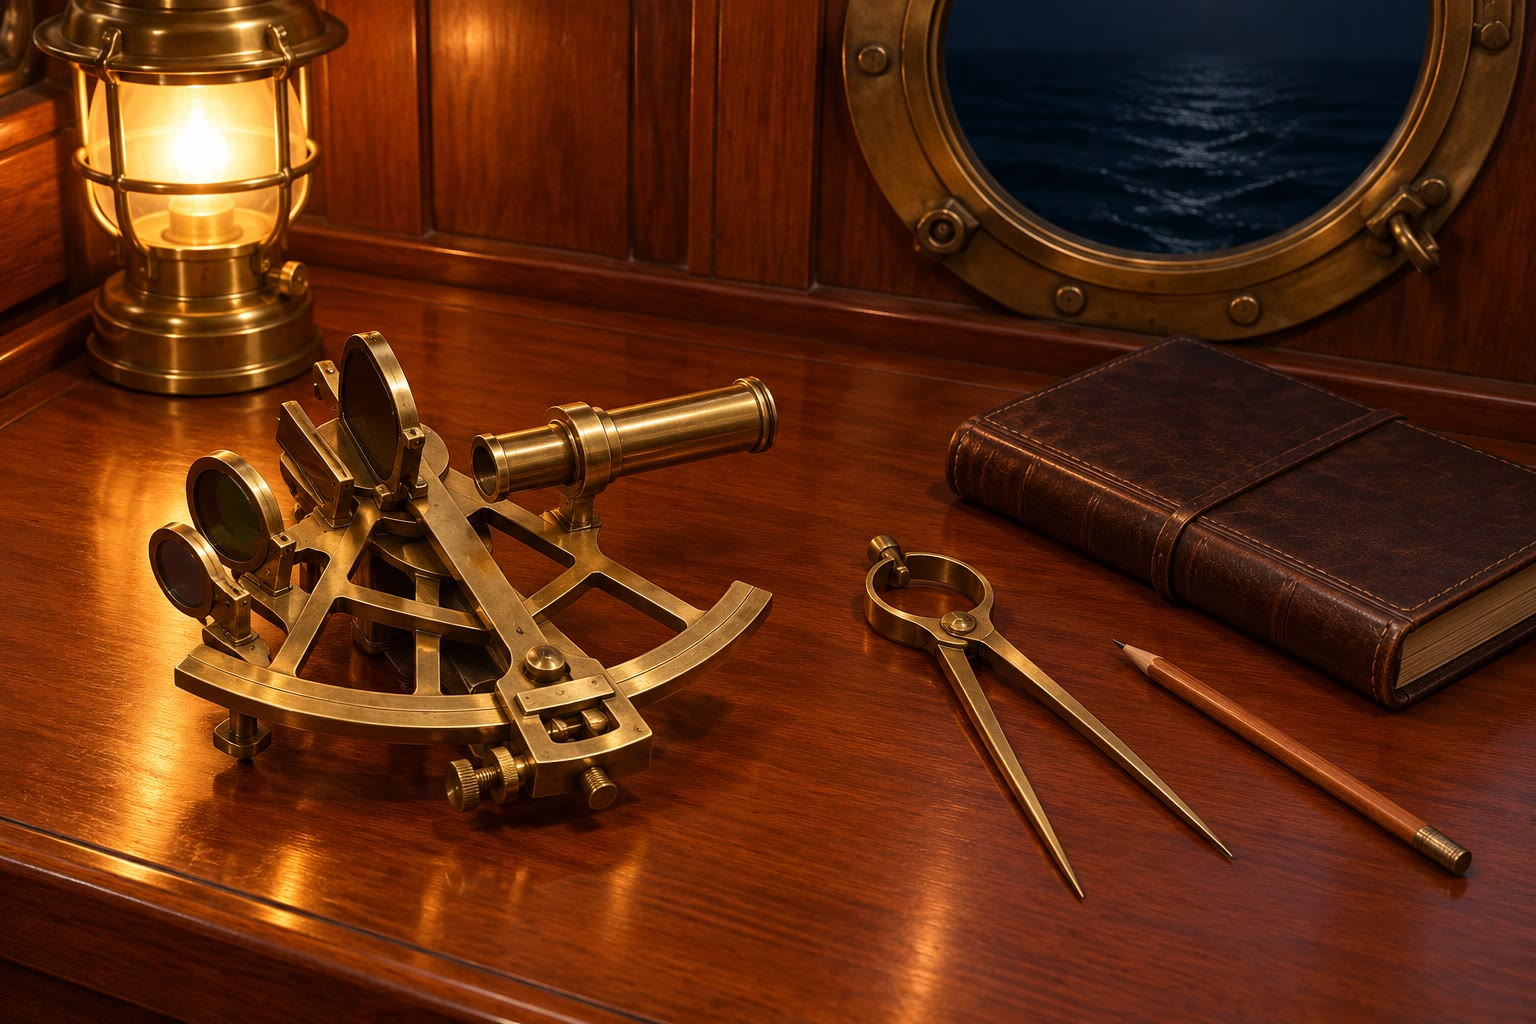
\includegraphics[width=0.55\linewidth]{images/book3/ai/b1-sextant.jpg}
\end{center}
\end{inthefield}

\section{Latihan}

\begin{exercise}[$\star$]\label{exo:b1:spherical-astronomy:1}
Seorang pengamat berada pada \omterm{def:b1:spherical-astronomy:geographic}{lintang} \ang{52} LU. Pada tinggi berapakah \omterm{def:b1:spherical-astronomy:celestial-sphere}{kutub langit} utara berada? Bintang-bintang mana, menurut deklinasinya, yang tidak pernah terbenam di sana, dan mana yang tidak pernah terbit?
\end{exercise}

\begin{exercise}[$\star$]\label{exo:b1:spherical-astronomy:2}
Ubah \omterm{def:b1:spherical-astronomy:equatorial}{asensio rekta} sebesar \qty{6}{h}~\qty{45}{min} ke dalam derajat. Pada \omterm{def:b1:spherical-astronomy:sidereal-time}{waktu sideris} setempat \qty{10}{h}~\qty{0}{min}, berapakah \omterm{def:b1:spherical-astronomy:equatorial}{sudut jam} bintang yang memiliki \omterm{def:b1:spherical-astronomy:equatorial}{asensio rekta} tersebut? Apakah bintang itu berada di timur atau di barat meridian?
\end{exercise}

\begin{exercise}[$\star$]\label{exo:b1:spherical-astronomy:3}
Pada \omterm{def:b1:spherical-astronomy:geographic}{lintang} \ang{40} LU, hitung \omterm{def:b1:spherical-astronomy:horizontal}{tinggi Matahari} pada tengah hari untuk kedua solstis dan untuk ekuinoks ($\varepsilon = \ang{23.44}$).
\end{exercise}

\begin{exercise}[$\star$]\label{exo:b1:spherical-astronomy:4}
Apakah tahun 1900 kabisat? Apakah tahun 2000? Akankah tahun 2100 kabisat? Dengan berapa hari per abad kalender Julius menyimpang dari \omterm{def:b1:spherical-astronomy:tropical-year}{tahun tropis} 365.2422 hari, dan berapa hari kalender Gregorius?
\end{exercise}

\begin{exercise}[$\star\star$]\label{exo:b1:spherical-astronomy:5}
Dua titik terletak pada \omterm{def:b1:spherical-astronomy:geographic}{lintang} \ang{45} LU, pada \omterm{def:b1:spherical-astronomy:geographic}{bujur} \ang{0} dan \ang{90} BT. Hitung jarak \omterm{def:b1:spherical-astronomy:spherical-triangle}{lingkaran besar} di antara keduanya ($R = \qty{6371}{km}$) dan jarak sepanjang paralelnya. Mana yang lebih pendek, dan dengan berapa?
\end{exercise}

\begin{exercise}[$\star\star$]\label{exo:b1:spherical-astronomy:6}
Pada \omterm{def:b1:spherical-astronomy:geographic}{lintang} \ang{48} LU, sebuah bintang dengan deklinasi \ang{20} memiliki \omterm{def:b1:spherical-astronomy:equatorial}{sudut jam} \ang{30}. Hitung tinggi dan \omterm{def:b1:spherical-astronomy:horizontal}{azimutnya}. Ke arah mana pengamat harus memandang?
\end{exercise}

\begin{exercise}[$\star\star$]\label{exo:b1:spherical-astronomy:7}
Hitung panjang hari pada \omterm{def:b1:spherical-astronomy:geographic}{lintang} \ang{60} LU saat solstis Juni, dengan Matahari dianggap sebagai titik pada horizon geometris. Periksa hasilmu pada gambar panjang hari.
\end{exercise}

\begin{exercise}[$\star\star$]\label{exo:b1:spherical-astronomy:8}
Sebuah bintang melintasi meridian malam ini pukul 22.00 \omterm{def:b1:spherical-astronomy:solar-time}{waktu matahari rata-rata} setempat. Pada pukul berapakah ia akan melintasi meridian dalam 30 hari? Dalam berapa hari ia akan melintas pada tengah hari, tak terlihat dalam cahaya siang?
\end{exercise}

\begin{exercise}[$\star\star$]\label{exo:b1:spherical-astronomy:9}
Hitung \omterm{def:b1:spherical-astronomy:insolation}{insolasi} di puncak atmosfer pada tengah hari di \omterm{def:b1:spherical-astronomy:geographic}{lintang} \ang{45} LU (a) pada salah satu ekuinoks, dengan $r = a$; (b) pada solstis Juni, dengan mengambil jarak aphelion untuk $r$. Data: $S_0 = \qty{1361}{W.m^{-2}}$, $a = \qty{149.598e6}{km}$, aphelion \qty{152.100e6}{km}.
\end{exercise}

\begin{exercise}[$\star\star\star$]\label{exo:b1:spherical-astronomy:10}
Dengan memakai \cref{prop:b1:spherical-astronomy:sun-declination}, hitung deklinasi dan \omterm{def:b1:spherical-astronomy:equatorial}{asensio rekta} Matahari ketika \omterm{def:b1:spherical-astronomy:geographic}{bujur} \omterm{def:b1:spherical-astronomy:ecliptic}{ekliptikanya} \ang{60}. Berapa derajat \omterm{def:b1:spherical-astronomy:equatorial}{asensio rekta} tertinggal di belakang \omterm{def:b1:spherical-astronomy:geographic}{bujur}? Jelaskan dengan hasil ini mengapa \omterm{def:b1:spherical-astronomy:ecliptic}{kemiringan ekliptika} ikut berkontribusi pada \omterm{def:b1:spherical-astronomy:solar-time}{perata waktu}.
\end{exercise}

\begin{exercise}[$\star\star\star$]\label{exo:b1:spherical-astronomy:11}
Tunjukkan bahwa pada solstis Juni Matahari terbit pada \omterm{def:b1:spherical-astronomy:horizontal}{azimut} $\mathrm{A}_0$ dengan $\cos\mathrm{A}_0 = \sin\varepsilon/\cos\varphi$. Pada \omterm{def:b1:spherical-astronomy:geographic}{lintang} berapakah ia terbit tepat di timur laut? Apa yang terjadi pada rumus ini di \omterm{def:b1:spherical-astronomy:geographic}{lintang} di atas $\ang{90} - \varepsilon$?
\end{exercise}

\begin{exercise}[$\star\star\star$]\label{exo:b1:spherical-astronomy:12}
Baji bola adalah bagian bola yang terletak di antara dua setengah \omterm{def:b1:spherical-astronomy:spherical-triangle}{lingkaran besar} yang menghubungkan dua titik berseberangan, dengan sudut $\theta$ satu sama lain. (a) Tunjukkan bahwa luasnya adalah $2\theta R^2$. (b) Setiap sisi \omterm{def:b1:spherical-astronomy:spherical-triangle}{segitiga bola} $ABC$, jika diperpanjang menjadi \omterm{def:b1:spherical-astronomy:spherical-triangle}{lingkaran besar} penuh, bersama sisi-sisi lain membentuk tiga pasang baji berseberangan dengan sudut $A$, $B$, $C$ yang menutupi bola; segitiga dan segitiga seberangnya tertutup tiga kali. Turunkan teorema Girard: luas segitiga adalah $R^2(A + B + C - \pi)$. (c) Terapkan hasil itu pada segitiga dengan tiga sudut siku-siku, dan pada segitiga yang digambar dalam bab ini (sudut \ang{89.9}, \ang{64.9}, \ang{67.4}).
\end{exercise}

\section{Soal: Semalam di observatorium gunung}

\begin{problem}[{Soal akhir pekan --- di mana Observatorium Paranal berdiri, apa yang tampak di langitnya, dan berapa lama malam terpanjangnya}]
\label{pb:b1:spherical-astronomy:1}
% ledger: mpc:paranal, mpc:greenwich, simbad:sirius, simbad:canopus, usno:seasons-2026, earth:obliquity, usno:tropical-year
% numbers computed in the scratch calculator calc/ch01.py from the rounded data
Observatorium Paranal berdiri di gurun Atacama pada \omterm{def:b1:spherical-astronomy:geographic}{lintang} \ang{24.63} LS, \omterm{def:b1:spherical-astronomy:geographic}{bujur} \ang{70.40} BB. Observatorium Kerajaan di Greenwich, tempat \omterm{def:b1:spherical-astronomy:geographic}{bujur} dihitung, berada pada \ang{51.48} LU, \ang{0.00}. Dua bintang terang di langit selatan memiliki koordinat
\begin{center}
\small
\begin{tabular}{lcc}
\hline
bintang & \omterm{def:b1:spherical-astronomy:equatorial}{asensio rekta} & deklinasi \\
\hline
Sirius & \qty{6}{h}~\qty{45}{min}~\qty{9}{s} & \ang{-16.72} \\
Canopus & \qty{6}{h}~\qty{23}{min}~\qty{57}{s} & \ang{-52.70} \\
\hline
\end{tabular}
\end{center}
Ambil $R = \qty{6371}{km}$, $\varepsilon = \ang{23.44}$, \omterm{def:b1:spherical-astronomy:tropical-year}{tahun tropis} 365.2422 hari, dan anggap Matahari sebagai titik pada horizon geometris.

\medskip
\noindent\textbf{Bagian I --- Paranal di permukaan Bumi.}
\begin{enumerate}
  \item Tentukan kolatitud Paranal dan Greenwich, serta selisih \omterm{def:b1:spherical-astronomy:geographic}{bujur} keduanya.
  \item Tuliskan aturan kosinus untuk segitiga Kutub Utara--Paranal--Greenwich, lalu hitung kosinus jarak sudut $\Delta$ antara kedua observatorium.
  \item Turunkan $\Delta$ dalam derajat dan jarak \omterm{def:b1:spherical-astronomy:spherical-triangle}{lingkaran besar} dalam kilometer.
  \item Hitung arah awal dari Paranal menuju Greenwich (\cref{met:b1:spherical-astronomy:great-circle}).
  \item Periksa arah itu dengan aturan sinus.
  \item Apakah pesawat yang mempertahankan arah ini sepanjang perjalanan akan mencapai Greenwich? Jelaskan.
\end{enumerate}

\medskip
\noindent\textbf{Bagian II --- Langit Paranal.}
\begin{enumerate}[resume]
  \item Pada tinggi berapakah \omterm{def:b1:spherical-astronomy:celestial-sphere}{kutub langit} selatan berada di atas cakrawala selatan Paranal?
  \item Pada tinggi berapakah Sirius melintasi meridian, dan di sisi \omterm{def:b1:spherical-astronomy:celestial-sphere}{zenit} manakah?
  \item Di bawah deklinasi berapakah sebuah bintang bersifat sirkumpolar di Paranal? Apakah Canopus sirkumpolar?
  \item Berapakah tinggi tertinggi yang dicapai Canopus?
  \item Hitung \omterm{def:b1:spherical-astronomy:equatorial}{sudut jam} saat Sirius terbit, dan berapa lama ia tetap di atas cakrawala, dalam jam sideris.
  \item Pada \omterm{def:b1:spherical-astronomy:horizontal}{azimut} berapakah Sirius terbit?
\end{enumerate}

\medskip
\noindent\textbf{Bagian III --- Jam.}
\begin{enumerate}[resume]
  \item Berapakah \omterm{def:b1:spherical-astronomy:sidereal-time}{waktu sideris} setempat ketika Sirius melintasi meridian?
  \item Hitung panjang hari sideris, dan berapa menit lebih awal lintasan meridian sebuah bintang setiap malam.
  \item Anggap \omterm{def:b1:spherical-astronomy:sidereal-time}{waktu sideris} setempat pada tengah malam \omterm{def:b1:spherical-astronomy:solar-time}{waktu matahari rata-rata} sebesar \qty{12}{h} pada ekuinoks Maret (20 Maret 2026), ketika Matahari berada dekat \omterm{def:b1:spherical-astronomy:ecliptic}{titik ekuinoks musim semi}; setelah itu \omterm{def:b1:spherical-astronomy:sidereal-time}{waktu sideris} bertambah $24/365.2422$ jam setiap hari. Berapa hari setelah ekuinoks Sirius melintasi meridian pada tengah malam \omterm{def:b1:spherical-astronomy:solar-time}{waktu matahari rata-rata}? Pada tanggal berapakah itu?
  \item Pada malam itu, berapa beda \omterm{def:b1:spherical-astronomy:solar-time}{waktu matahari rata-rata} di Paranal dengan waktu di Greenwich?
  \item \omterm{def:b1:spherical-astronomy:solar-time}{Perata waktu} saat itu sekitar \qty{-3}{min}. Pukul berapakah jam matahari di observatorium menunjukkan (\omterm{def:b1:spherical-astronomy:solar-time}{waktu matahari semu}) ketika Sirius melintasi meridian?
  \item Berapa lama lebih awal ia melintasi meridian seminggu kemudian?
\end{enumerate}

\medskip
\noindent\textbf{Bagian IV --- Malam terpanjang.}
\begin{enumerate}[resume]
  \item Berapakah deklinasi Matahari pada setiap solstis?
  \item Hitung \omterm{def:b1:spherical-astronomy:horizontal}{tinggi Matahari} pada tengah hari di Paranal pada solstis Juni dan solstis Desember. Di sisi \omterm{def:b1:spherical-astronomy:celestial-sphere}{zenit} manakah ia berada pada bulan Desember?
  \item Pada solstis Desember jarak Matahari--Bumi adalah 0.9837 kali jarak rata-rata. Hitung \omterm{def:b1:spherical-astronomy:insolation}{insolasi} pada tengah hari di puncak atmosfer di atas Paranal ($S_0 = \qty{1361}{W.m^{-2}}$).
  \item Pada solstis yang mana malam di Paranal paling panjang? Hitung \omterm{def:b1:spherical-astronomy:equatorial}{sudut jam} saat matahari terbenam pada tanggal itu.
  \item Pada \omterm{def:b1:spherical-astronomy:horizontal}{azimut} berapakah Matahari terbit pada tanggal itu?
  \item Turunkan panjang malam terpanjang dalam setahun di Paranal, dalam jam dan menit.
\end{enumerate}
\end{problem}
